\appendix


\section{Additional Experimental Results}
\label{sec:appendix_results}

This appendix provides detailed experimental results that supplement the main paper.


\subsection{Fast-dLLM-v2-7B Results}
\label{app:additional_results}

Figure~\ref{fig:longbench_7b} presents per-task accuracy results on LongBench for Fast-dLLM 7B. Similar to the 1.5B model results in the main paper, MAGE consistently outperform Quest and Tidal across all tasks and budget settings.

Figure~\ref{fig:latency_7B} presents per-task per-step latency results on LongBench for Fast-dLLM 7B.

\begin{figure*}[h]
    \centering
    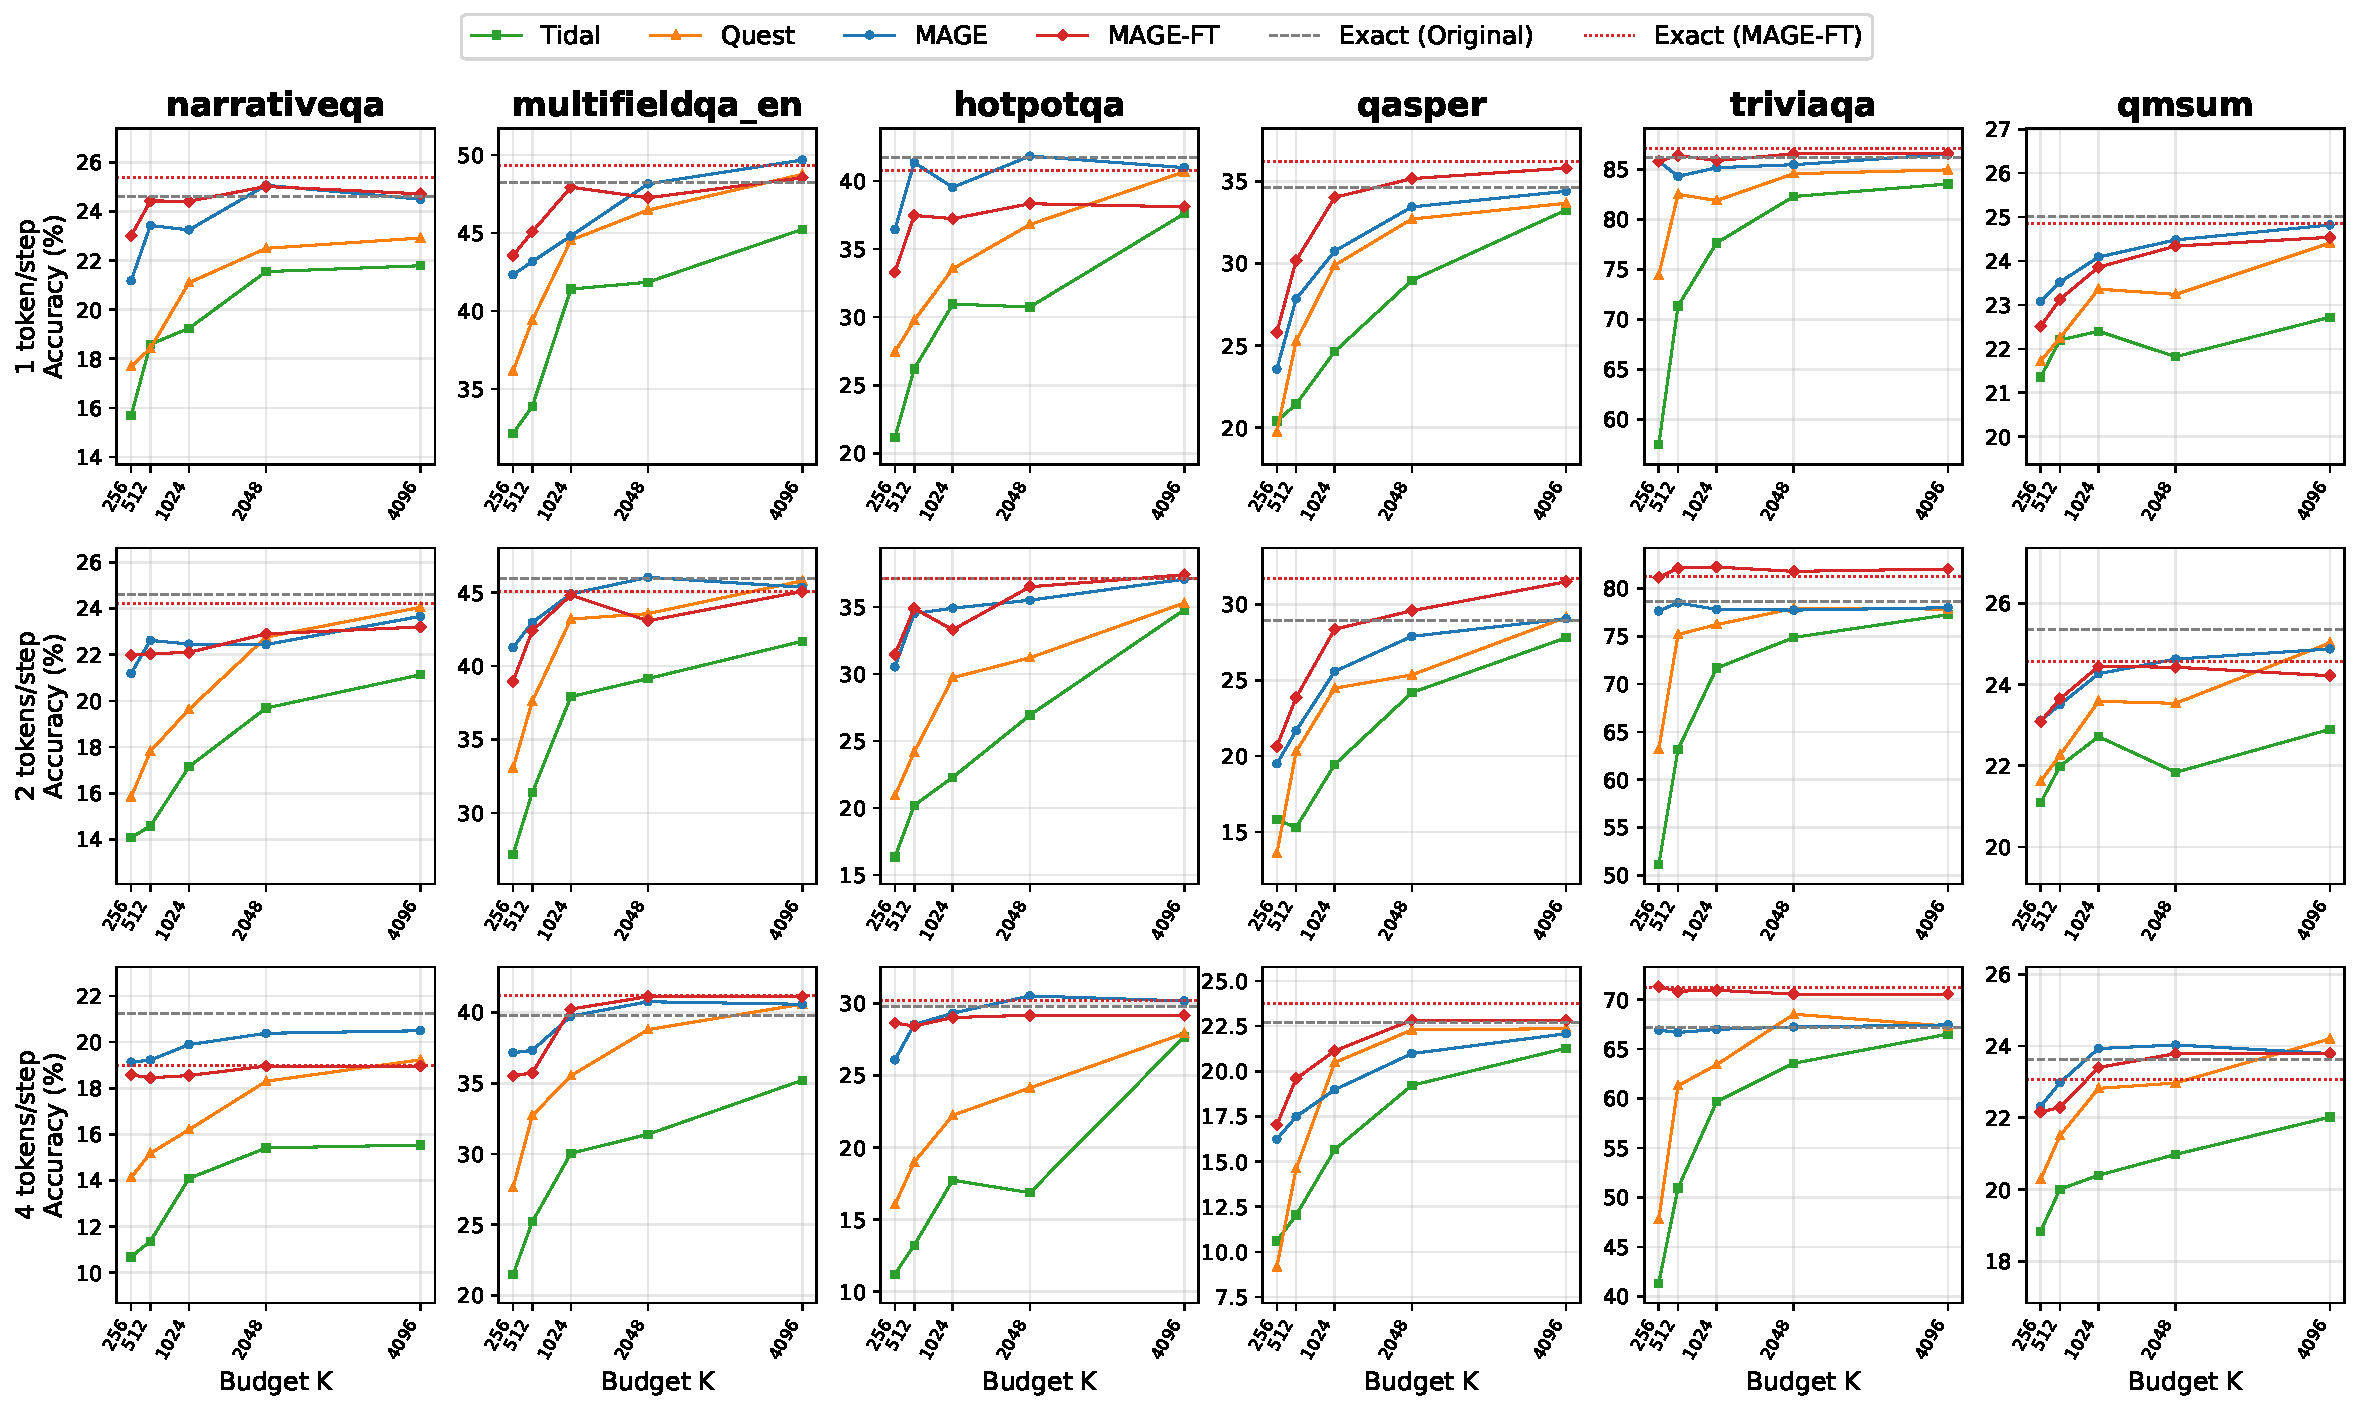
\includegraphics[width=0.80\linewidth]{figures/fig5_7b_acc_static_combined.pdf}
    \caption{Per-task accuracy on LongBench with Fast-dLLM 7B across varying budget $K$.}
    \label{fig:longbench_7b}
\end{figure*}
\begin{figure*}[h]
    \centering
    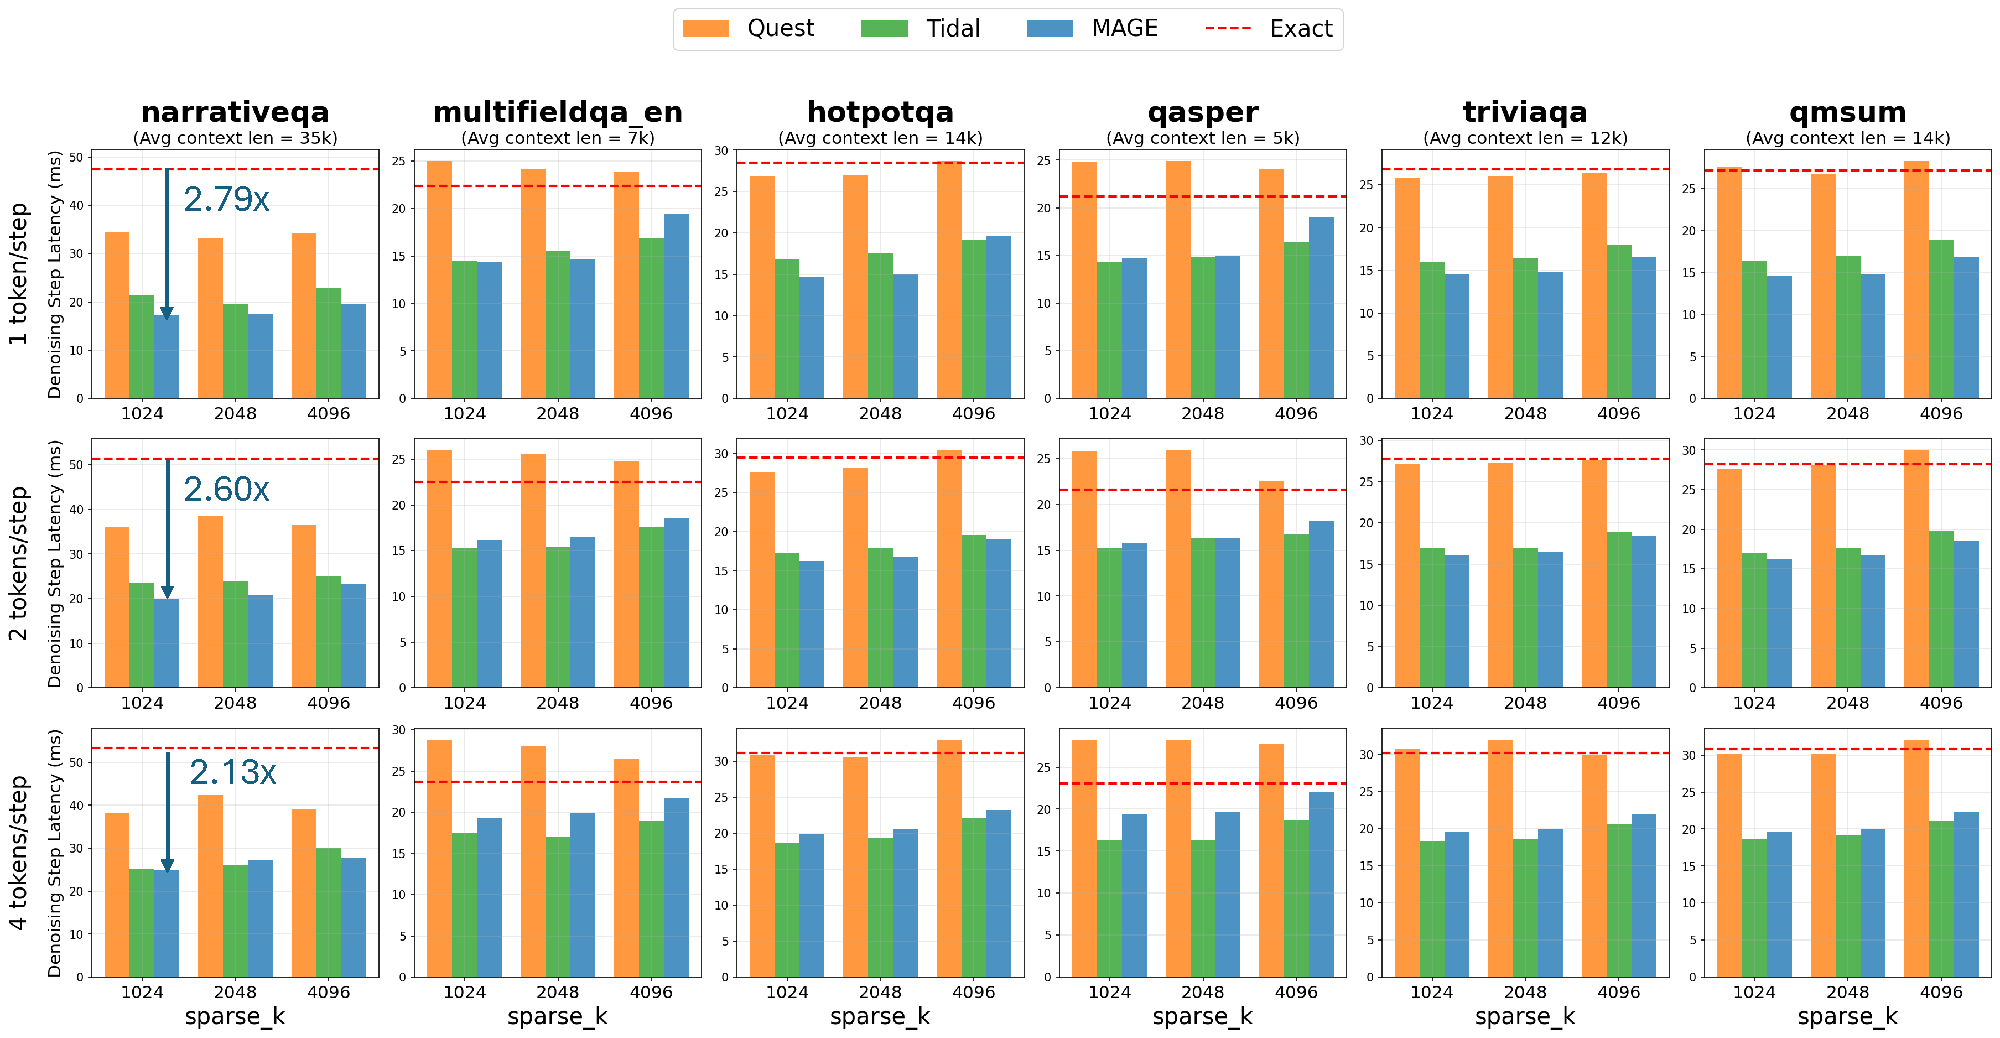
\includegraphics[width=0.80\linewidth]{figures/fig8_avg_latency_per_step_7B.pdf}
    \caption{Per-task average denoising step latency on LongBench with Fast-dLLM 7B across three denoising configurations (1, 2, 4 tokens/step).}
    \label{fig:latency_7B}
\end{figure*}


\clearpage

\subsection{Baseline Sparse Attention Methods' Top-K Recall Rate}
\label{sec:baseline_sparse_methods}
\begin{figure}[h]
    \centering
    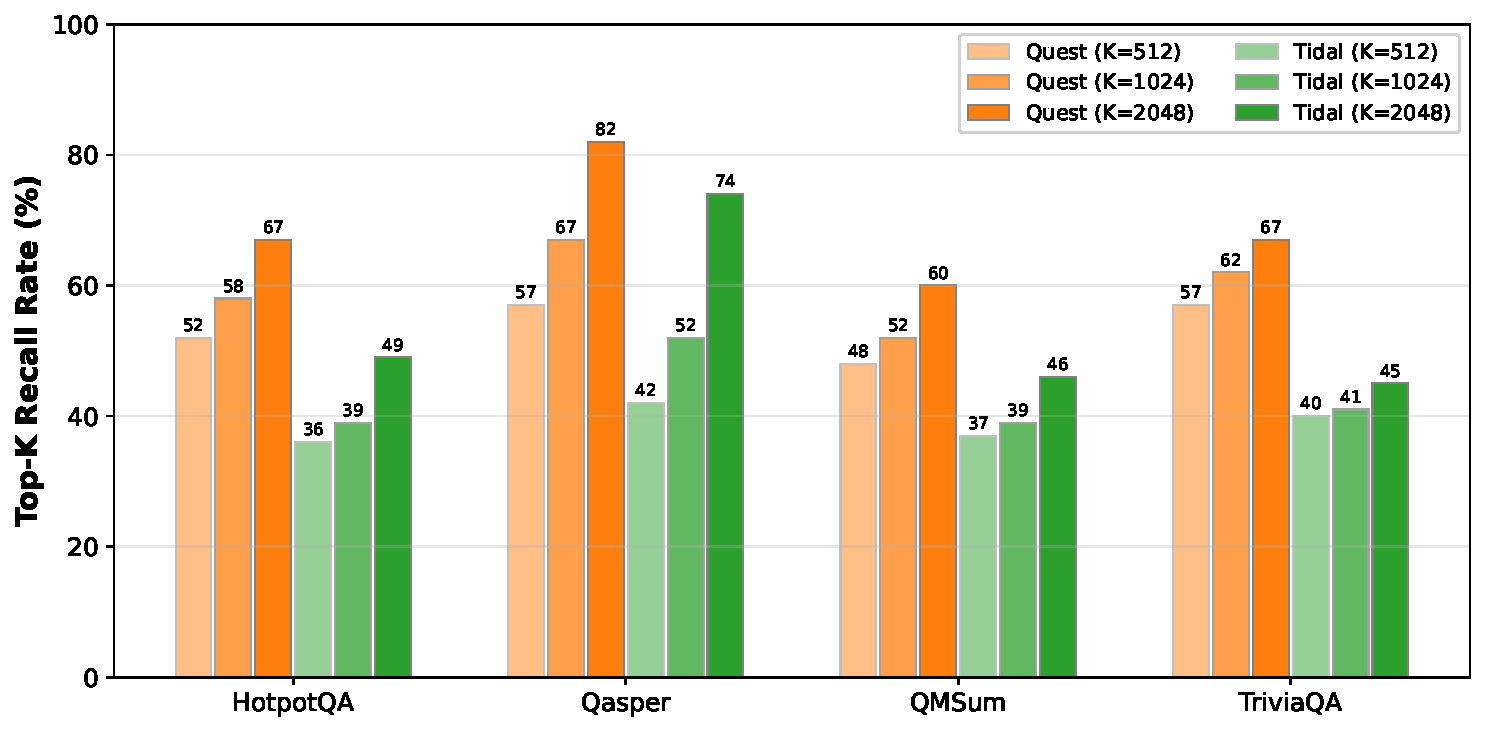
\includegraphics[width=0.9\linewidth]{figures/fig2_method_comparison.pdf}
    \caption{Top-K recall rate of different sparse attention strategies adapted to block diffusion. Quest (48--82\%) and Tidal (36--74\%) achieve limited recall, while All-\mask-guided selection maintains 84--90\%.}
    \label{fig:method_comparison}
\end{figure}

\subsection{Ablation Study: Layer-Adaptive Budget Redistribution}
\label{app:ablation}

Tables~\ref{tab:ablation_sidebyside} present ablation results comparing MAGE (step reuse only) and MAGE+ (with layer-adaptive budget redistribution). Values show MAGE+ accuracy with the difference from MAGE in parentheses. \textcolor{blue}{Blue (+)} indicates improvement from layer-adaptive budgets, while \textcolor{red}{red (--)} indicates degradation.

Overall, layer-adaptive budget redistribution provides modest improvements on average, particularly benefiting retrieval-heavy tasks like HotpotQA.

% Stacked Ablation Table: 1.5B and 7B, 32 steps
\begin{table}[h]
\centering
\small
\caption{Effect of layer-adaptive budget redistribution (32 denoising steps). Values show MAGE+ accuracy with difference from MAGE in parentheses.}
\label{tab:ablation_sidebyside}
\begin{tabular*}{\columnwidth}{@{\extracolsep{\fill}}l|ccccc}
\toprule
\multicolumn{6}{c}{\textbf{Fast-dLLM 1.5B}} \\
\midrule
Task & 256 & 512 & 1K & 2K & 4K \\
\midrule
NarrativeQA & 12.8 (\textcolor{blue}{+0.4}) & 11.9 (\textcolor{red}{-0.6}) & 12.2 (\textcolor{blue}{+0.2}) & 12.8 (\textcolor{red}{-0.6}) & 12.4 (\textcolor{blue}{+0.4}) \\
MultiFieldQA & 32.8 (\textcolor{red}{-0.2}) & 33.7 (\textcolor{blue}{+0.7}) & 34.4 (\textcolor{red}{-1.9}) & 38.4 (\textcolor{blue}{+0.1}) & 38.2 (\textcolor{blue}{+0.2}) \\
HotpotQA & 14.7 (\textcolor{red}{-0.4}) & 14.5 (\textcolor{blue}{+0.3}) & 14.3 (\textcolor{blue}{+0.9}) & 13.5 (\textcolor{red}{-0.9}) & 15.7 (\textcolor{blue}{+0.2}) \\
Qasper & 13.3 (\textcolor{blue}{+0.1}) & 16.3 (\textcolor{red}{-0.3}) & 19.0 (\textcolor{blue}{+0.9}) & 20.6 (\textcolor{blue}{+0.3}) & 19.7 (\textcolor{red}{-0.7}) \\
TriviaQA & 64.1 (\textcolor{blue}{+1.0}) & 65.6 (\textcolor{blue}{+0.2}) & 69.3 (\textcolor{blue}{+1.6}) & 71.1 (\textcolor{blue}{+0.7}) & 70.5 (\textcolor{blue}{+0.4}) \\
QMSum & 21.5 (\textcolor{red}{-0.3}) & 21.9 (\textcolor{red}{-0.2}) & 22.8 (\textcolor{blue}{+0.1}) & 23.5 (\textcolor{blue}{+0.4}) & 23.2 (\textcolor{blue}{+0.2}) \\
\bottomrule
\end{tabular*}
\vspace{0.5em}
\begin{tabular*}{\columnwidth}{@{\extracolsep{\fill}}l|ccccc}
\toprule
\multicolumn{6}{c}{\textbf{Fast-dLLM 7B}} \\
\midrule
Task & 256 & 512 & 1K & 2K & 4K \\
\midrule
NarrativeQA & 21.2 (\textcolor{blue}{+0.3}) & 23.4 (\textcolor{blue}{+0.0}) & 23.2 (\textcolor{red}{-0.7}) & 25.1 (\textcolor{red}{-0.8}) & 24.5 (\textcolor{red}{-0.8}) \\
MultiFieldQA & 42.3 (\textcolor{blue}{+1.1}) & 43.2 (\textcolor{blue}{+0.3}) & 44.8 (\textcolor{red}{-1.2}) & 48.1 (\textcolor{blue}{+0.2}) & 49.7 (\textcolor{blue}{+0.1}) \\
HotpotQA & 36.4 (\textcolor{blue}{+0.3}) & 41.4 (\textcolor{blue}{+1.6}) & 39.5 (\textcolor{blue}{+1.0}) & 41.8 (\textcolor{blue}{+1.8}) & 41.0 (\textcolor{blue}{+0.9}) \\
Qasper & 23.6 (\textcolor{red}{-0.9}) & 27.8 (\textcolor{blue}{+1.8}) & 30.8 (\textcolor{blue}{+0.1}) & 33.4 (\textcolor{blue}{+0.1}) & 34.4 (\textcolor{blue}{+0.3}) \\
TriviaQA & 85.8 (\textcolor{blue}{+0.4}) & 84.3 (\textcolor{blue}{+0.0}) & 85.2 (\textcolor{red}{-0.2}) & 85.5 (\textcolor{red}{-0.1}) & 86.5 (\textcolor{red}{-0.2}) \\
QMSum & 23.1 (\textcolor{red}{-0.4}) & 23.5 (\textcolor{blue}{+0.2}) & 24.1 (\textcolor{blue}{+0.0}) & 24.5 (\textcolor{blue}{+0.4}) & 24.8 (\textcolor{blue}{+0.3}) \\
\bottomrule
\end{tabular*}
\end{table}

\clearpage

\subsection{Extended Breakdown Analysis}
\label{app:breakdown}

\begin{figure}[h]
    \centering
    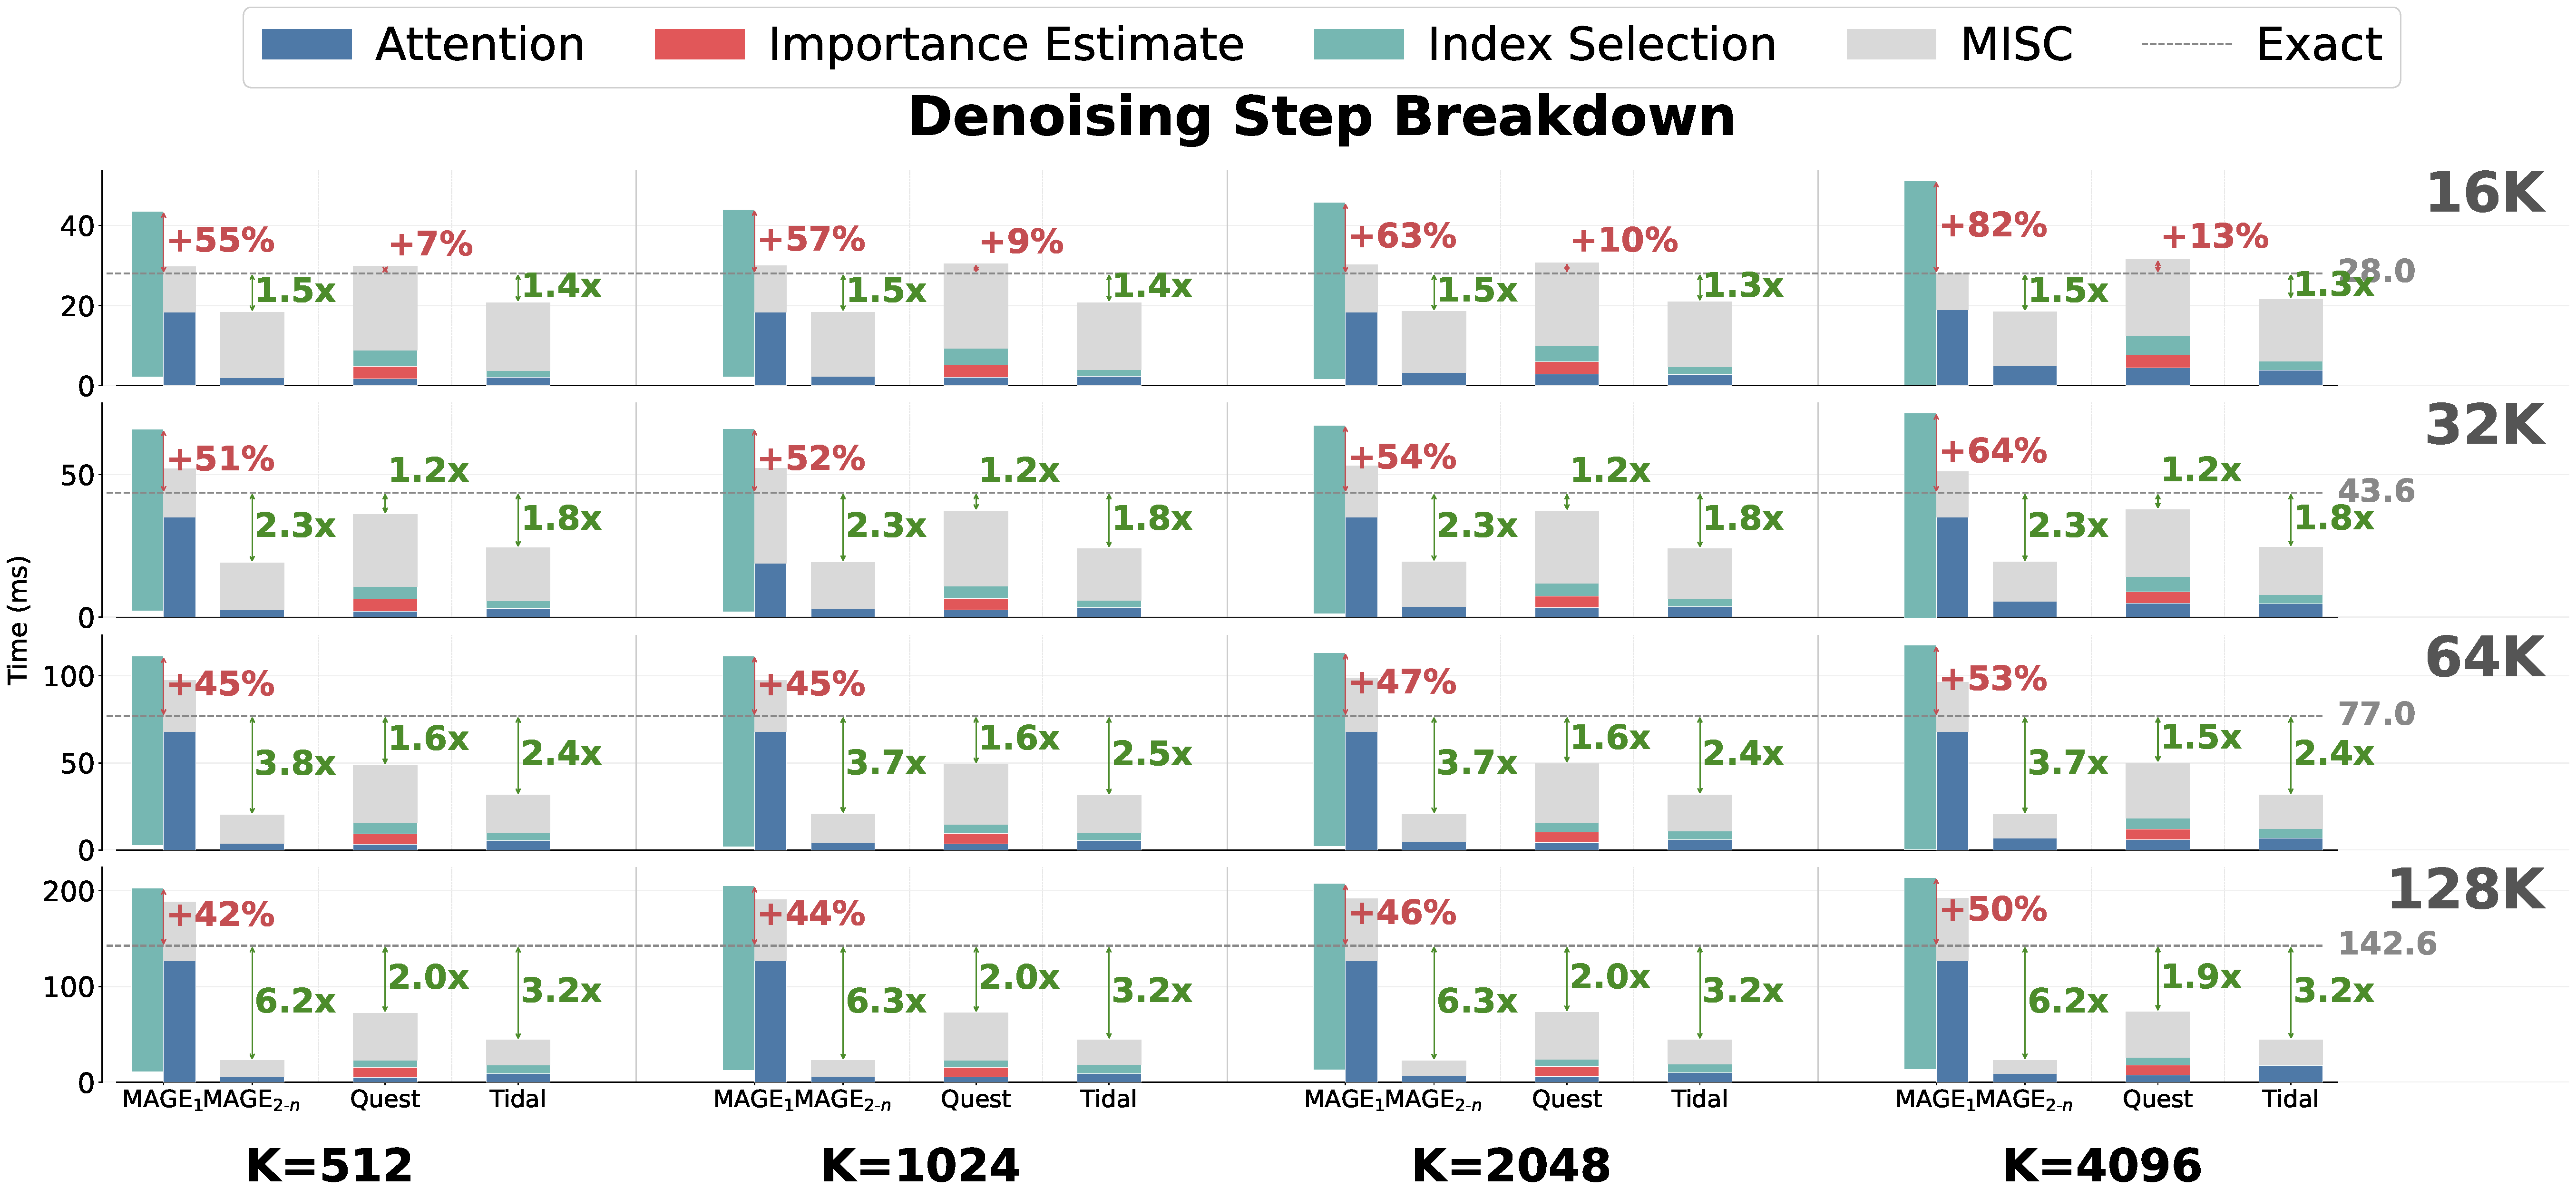
\includegraphics[width=0.9\linewidth]{figures/breakdown.pdf}
    \caption{Complete denoising step latency breakdown across context lengths (16K--128K) and top-$k$ values (512, 1024, 2048, 4096). 
    Each group compares Exact attention, Quest, TidalDecode, and MAGE (first step MAGE$_1$ and subsequent steps MAGE$_{2\text{-}n}$).
    For MAGE$_1$, stacked bars show overlapped (left) and main-stream (right) operations.
    Dashed lines indicate exact attention latency as baseline; numbers denote relative speedup ($>$1$\times$) or overhead ($<$1$\times$).}
    \label{fig:breakdown_full}
\end{figure}

Figure~\ref{fig:breakdown_full} extends the breakdown analysis from Section~\ref{subsec:efficiency} across all $K$ configurations.
We observe consistent trends across different $K$ values:


\section{Implementation Details}
\label{appendix:implementation}

This section describes the optimization techniques employed to achieve efficient sparse attention in Block Diffusion LLMs. 
All optimizations are applied uniformly across all baseline methods to ensure fair comparison.

\subsection{Sparse Attention Kernel Optimization}
\label{appendix:kernel_opt}
We build our sparse attention kernel by extending the implementations 
from TidalDecode~\cite{yang2025tidaldecode} and Quest~\cite{tang2024quest}, 
which utilize FlashInfer~\cite{ye2025flashinfer} for paged KV cache 
management with indirect indexing.

The original implementations target autoregressive (AR) decoding, where the query sequence length is always one. 
To support Block Diffusion models that process multiple query tokens simultaneously, we extend the prefill kernel with the following modifications:
\begin{itemize}
    \item \textbf{Fixed query length support:} The original decode kernels only support query length of one. We extend them to support power-of-two query lengths (e.g., 8, 16, 32) used in block-parallel decoding.
    \item \textbf{GQA-compatible sparse attention:} We modify the kernel to allow each KV head group to access different sparse indices, enabling sparse attention with Grouped-Query Attention (GQA).
\end{itemize}

\subsection{Fused Kernel for Union Formation}
\label{appendix:fused_kernel}

When the KV cache length becomes large, even simple operations such as \texttt{reshape} and \texttt{copy} incur significant overhead due to memory movement. 
To minimize these costs, we design fused Triton kernels for the Union Formation operation described in Section~\ref{sec:method}.

Since the tensor shapes remain constant across decoding steps, we exploit this property to pre-compile specialized kernels that:
\begin{itemize}
    \item Eliminate intermediate memory allocations
    \item Fuse multiple element-wise operations into a single kernel launch
    \item Minimize memory transactions by operating in-place where possible
\end{itemize}

\subsection{Multi-Stream Execution}
\label{appendix:multistream}

\begin{figure}[t]
    \centering
    \includegraphics[width=\linewidth]{figures/multistream.pdf}
    \caption{Comparison of attention scheduling strategies within a single denoising step. 
    Quest alternates between importance estimation (Est.) and sparse (Sp.) attention phases. 
    Tidal interleaves exact and sparse attention sequentially. 
    MAGE$_1$ (first step) performs exact attention on the main stream while asynchronously 
    computing Top-K indices for subsequent steps. 
    MAGE$_{2\text{-}n}$ leverages precomputed indices to execute sparse attention, 
    effectively hiding Top-K selection latency through cross-step pipelining.}
    \label{fig:multistream}
\end{figure}
In the decoding phase, most operations are memory-bound due to the small batch size. 
Additionally, our custom attention kernel is configured to use a limited number of streaming multiprocessors (SMs).
These characteristics enable effective overlap between independent operations through CUDA streams.

Unlike prior sparse attention methods, our approach allows for extensive pipelining. 
In TidalDecode, the top-$k$ selection result is immediately required by the next layer, creating a sequential dependency. 
Similarly, Quest must complete its attention score estimation before performing sparse attention within the same layer.
In contrast, our Union Formation and Index Selection operations for a given layer only need to complete before that layer begins in the \textit{next} denoising step, eliminating the intra-step dependency and enabling overlap with the current step's attention computation.

As illustrated in Figure~\ref{fig:multistream}, MAGE$_1$ computes exact attention while simultaneously preparing Top-$k$ indices on an asynchronous stream, and MAGE$_{2\text{-}n}$ directly utilizes these precomputed indices for sparse attention.
Specifically, we pipeline the Union Formation and Index Selection operations across multiple CUDA streams. 
Since these operations do not compete heavily for compute resources, they achieve substantial overlap with the attention computation.

Table~\ref{tab:overlap} demonstrates the effectiveness of multi-stream execution. 
We measure the overlap benefit as the difference between sequential execution time (Dense + Top-$k$) and the actual first-step latency.
The results show that multi-stream execution reduces the first-step latency by 30--40\% compared to sequential execution, with larger savings at longer context lengths.
For example, at 128K context with $K
$=512, overlap saves 127.17ms out of 330.02ms sequential time (38.5\% reduction).

\begin{table}[h]
\centering
\caption{Multi-stream overlap analysis. Each cell shows overlap savings in ms, with total first-step latency in parentheses.}
\label{tab:overlap}
\begin{tabular}{l|cccc}
\toprule
\textbf{Top-$k$} & \textbf{16K} & \textbf{32K} & \textbf{64K} & \textbf{128K} \\
\midrule
512  & 32.77 (43.56) & 41.29 (65.86) & 73.62 (111.26) & 127.17 (202.85) \\
1024 & 32.86 (44.05) & 41.81 (66.11) & 74.91 (111.43) & 126.99 (205.34) \\
2048 & 27.26 (45.72) & 42.41 (67.27) & 74.77 (113.32) & 126.65 (207.53) \\
4096 & 32.11 (51.16) & 46.78 (71.60) & 79.69 (117.57) & 129.32 (213.91) \\
\bottomrule
\end{tabular}
\end{table}

\subsection{Reducing Launch Overhead with CUDA Graph}
\label{appendix:cudagraph}

Although Block Diffusion decoding uses longer query sequences than standard autoregressive decoding, 
the operations remain memory-bound due to the large KV cache size.
These memory-bound operations complete quickly on the GPU, 
making CPU-side kernel launch overhead a significant bottleneck.

To address this, we employ CUDA Graphs to capture and replay the entire decoding step as a single graph execution. 
This eliminates per-kernel launch overhead and reduces CPU-GPU synchronization points, resulting in improved end-to-end latency.

\paragraph{Fair Comparison.}
All optimization techniques described above---kernel optimization, fused operations, and CUDA Graph---are applied consistently to all baseline methods evaluated in our experiments.
This ensures that performance differences reflect algorithmic improvements rather than implementation disparities.
Note that multi-stream execution is unique to our method due to the relaxed dependency structure, and thus represents a genuine algorithmic advantage.


